\documentclass[sigconf]{acmart}

\usepackage{booktabs} % For formal tables
\usepackage{listings} % For verbatim text (algorithms)


\definecolor{mGreen}{rgb}{0,0.6,0}
\definecolor{mGray}{rgb}{0.5,0.5,0.5}
\definecolor{mPurple}{rgb}{0.58,0,0.82}
\definecolor{backgroundColour}{rgb}{0.95,0.95,0.92}
\lstset{basicstyle=\footnotesize\ttfamily,breaklines=true}
\lstset{framextopmargin=50pt,frame=bottomline}
\lstdefinestyle{myStyle}{
    backgroundcolor=\color{backgroundColour},
    commentstyle=\color{mGreen},
    keywordstyle=\color{magenta},
    numberstyle=\tiny\color{mPurple},
    stringstyle=\color{mPurple},
    basicstyle=\footnotesize\ttfamily,
    breakatwhitespace=false,
    breaklines=true,
    captionpos=b,
    keepspaces=true,
    numbers=left,
    numbersep=5pt,
    showspaces=false,
    showstringspaces=false,
    showtabs=false,
    tabsize=2
}

\acmPrice{15.00}

% The next six lines come directly from the completed rights form.
% You MUST replace them with the lines specific to your accepted work.
\copyrightyear{2019}
\acmYear{2019}
\setcopyright{rightsretained}
\acmConference{}{}{}
\acmDOI{}
\acmISBN{}

% Use the "authoryear" citation style, and make sure citations are in [square brackets].
\citestyle{acmauthoryear}
\setcitestyle{square}

% A useful command for controlling the number of authors per row.
% The default value of "authorsperrow" is 2.
\settopmatter{authorsperrow=4}

% end of preamble.

\begin{document}

% Title.
% If your title is long, consider \title[short title]{full title} - "short title" will be used for running heads.
\title{Particle-in-cell Method for Incompressible Fluids}

% Authors.
\author{Jonathan Panuelos}
\affiliation{%
  \department{David R. Cheriton School of Computer Science}
  \institution{University of Waterloo}}
\email{jgpanuel@uwaterloo.ca}

% This command defines the author string for running heads.
\renewcommand{\shortauthors}{Panuelos}

% abstract
\begin{abstract}
Fluid simulation has long since been dominated by two competing formulations -- the Eulerian which computes fluid fluxes across a stationary reference frame, and the Lagrangian which advects particles with the fluid velocity. Each of these has its own strengths and weaknesses. Hybrid methods have been recently popularized to attempt to make use of each method's advantages while avoiding their problems. One such method is the Particle-in-Cell (PIC) method, which uses particles for advection and a background grid to apply forces and enforce incompressibility. We present an overview of the method, as well as its slight modification the Fluid-Implicit-Particle (FLIP) method. Finally, we demonstrate a simple 2D implementation written in C++, as well as comment on some of the results found.
\end{abstract}

%CCS
\begin{CCSXML}
<ccs2012>
<concept>
<concept_id></concept_id>
<concept_desc>Computing methodologies~Fluid Simulation</concept_desc>
<concept_significance>500</concept_significance>
</concept>
\end{CCSXML}

\ccsdesc[500]{Computing methodologies~Fluid Simulation}

%keywords
\keywords{particle in cell, material point, incompressible fluids}

% A "teaser" figure, centered below the title and authors and above the body of the work.
\begin{teaserfigure}
  \centering
  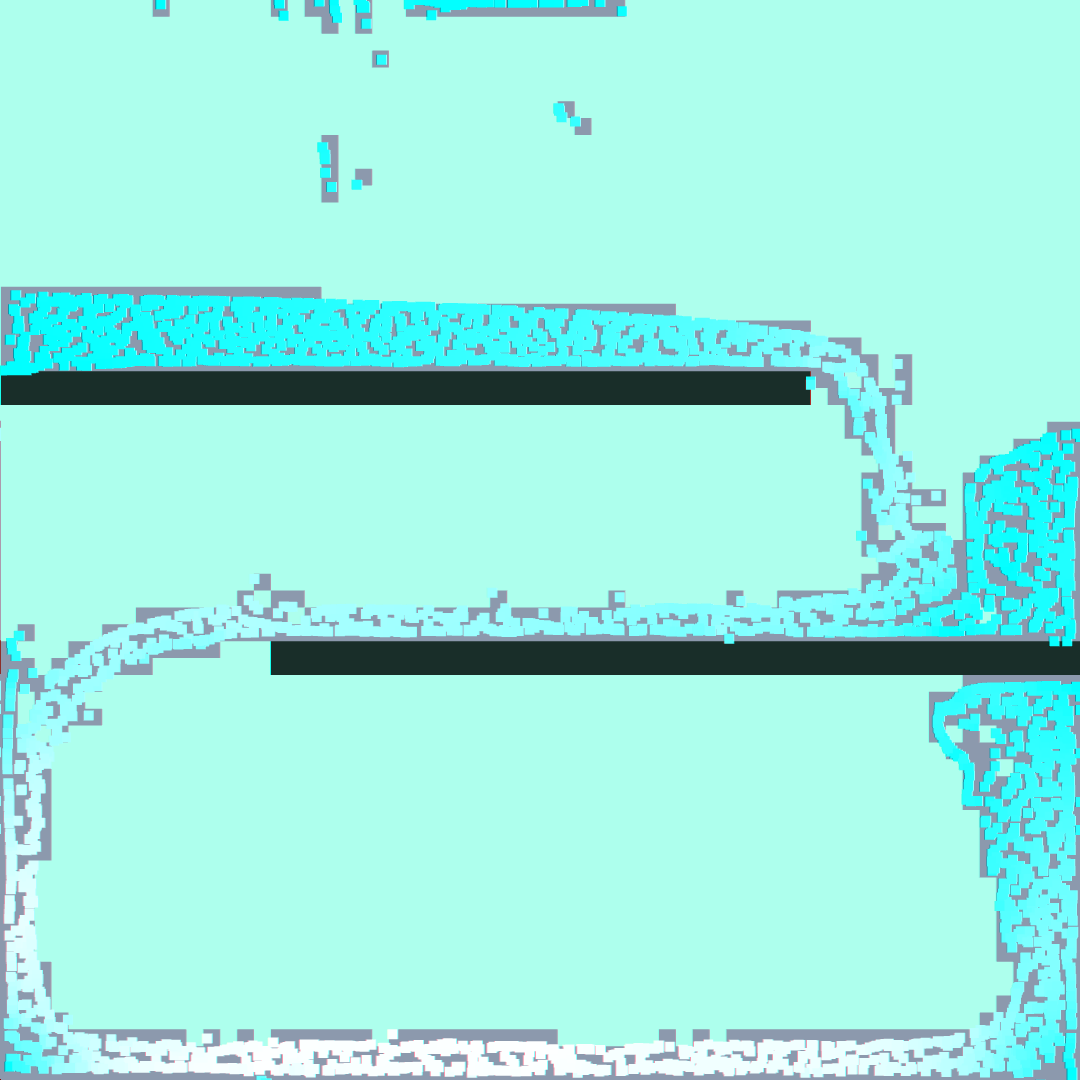
\includegraphics[width=3.0in]{img/Maze64.png}
  \caption{Fluid dropped on two planks at $t=1.5$ using the $\alpha{}=0.1$ PIC/FLIP blend on a $64\times{}64$ background grid with timestep size $\Delta{}t=0.001$.} \label{fig:teaser}
\end{teaserfigure}

% Processes all of the front-end information and starts the body of the work.
\maketitle

\section{Introduction}

Most numerical methods developed for computational fluid dynamics fall under two dominant categories derived from two different formulations of the fluid equations: Eulerian and Lagrangian methods. Eulerian methods take on the stationary reference frame by defining control volumes, often a regular grid, and computing fluid flux through them. Lagrangian methods use a moving reference frame that travels with the fluid velocity, advecting physical piece of matter over time. The two of these have competing advantages and disadvantages. The Eulerian grid allows for fast computation and potentially higher-order solvers, but at the expense of excessive diffusion due to accumulated averaging during the advection step. Lagrangian methods, on the other hand, have simple advection and free mass conservation, but at the expense of increased computational cost associated with nearest-neighbour searches, remeshing, and constricting stability conditions for the pressure solves \cite{zhu2005}.

Hybrid approaches attempt to make use of advantages and avoid weaknesses of either scheme. The Material Point Method (MPM) is one such scheme that uses Lagrangian particles to advect the fluid, but forces are solved using an Eulerian background grid \cite{JiangCourse}. We present a 2D implementation of two closely related flavours of MPM -- the Particle-in-Cell (PIC) method and the Fluid-Implicit-Particle (FLIP) method -- as well as the blended PIC/FLIP scheme. Our implementation largely follows from \cite{zhu2005}, which introduced PIC/FLIP into computer graphics, as well as from \cite{bridson2015}, which includes more implementation detail for basic grid-based fluid solvers. We present each step of the method, comment on our specific implementation, and demonstrate some results.

\section{Related Work}

\subsection{Grid and Particle Methods}

Grid methods have long been the standard for the numerical simulation of fluids -- the first grid-based fluid simulation was introduced by \cite{foster1996}. The natural implementation of finite differences into grids and associated computational efficiency make it attractive to the computer graphics field. The grid method we draw from uses a staggered MAC grid, as introduced by \cite{harlow1965}. By contrast, particle-based methods such as Smoothed Particle Hydrodynamics (SPH) forgo the grid, computing gradients using kernel functions. SPH was initially developed in the astrophysics literature by \cite{lucy1977, gingold1977}, and subsequently introduced into computer graphics by \cite{muller2003}.

\subsection{Hybrid Methods}

Material point methods has been a rich area of research in recent years, with various methods being introduced for fluids, as well as other materials such as deformable and granular solids. The first such method originates from early computational fluid dynamics, with the introduction of PIC \cite{harlow1962}. This method was built upon with a minor variation by Brackbill and Ruppel, replacing the direct velocity interpolation with incrementing the particle velocities using the interpolation of the change in velocity, creating the FLIP method \cite{brackbill1986}. Both methods were introduced into the field of computer graphics by Zhu and Bridson, who included a constitutive model to adapt it for simulating sand \cite{zhu2005}. This work pioneered the development of a wide range of similar hybrid methods in computer graphics based around particle advection and Eulerian fluid solves.

MPM was initially introduced by Stomakhin \emph{et. al.} 2013, who specifically applied it to snow \cite{stomakhin2013}, and is largely considered the generalization of the prior PIC and FLIP schemes. In particular, it introduces the application of a deformation gradient for computing elastic forces for deformable solids. This was later extended to include heat transfer and allow for materials undergoing phase-change \cite{stomakhin2014}.

Improvements to PIC came by way of the Affine Particle-in-Cell (APIC) method, which reintroduces lost angular momentum data in the interpolation steps \cite{jiang2015}; as well as the the Polynomial Particle-in-Cell (PolyPIC) method, which reintroduces higher order modes \cite{fu2017}. \cite{hu2018} introduced the use of the moving-least-squares interpolation to MPM as a generalization of APIC and PolyPIC.

\section{Method}

\subsection{Overview}

As prior stated, the PIC/FLIP method, and MPM in general, uses two fluid representations - a fundamental particle representation primarily used for advection, and a background grid for applying forces and enforcing incompressibility. Broadly, the PIC/FLIP method starts with the fluid represented as particles with positions and velocities. Fluid variables such as velocity are interpolated into the grid, which is then evolved over time. This grid step is effectively identical to any standard grid-based fluid solver but without the advection step. After the grid update, fluid properties are transferred back from the grid to the particles, which are then advected according to the particle velocities. We have the following general algorithm, adapted from \cite{zhu2005}:
\begin{lstlisting}[style=myStyle]
Initialize particle positions and velocities
For each timestep:
  Perform particle to grid interpolation.
  (FLIP) Save grid velocities.
  Perform standard grid fluid solve except for advection.
  (FLIP) Subtract new grid velocities from the saved grid velocities and increment particle velocities with the interpolated values.
  (PIC) Interpolate the new grid velocities directly into the particles.
  Advect particles.
  Detect and resolve solid boundary collisions.
  Adjust fluid surface representation.
\end{lstlisting}
Notice that much of the PIC and FLIP methods are taken directly from pre-existing grid and particle algorithms -- their defining characteristic are how the particle-to-grid and grid-to-particle interpolations are performed. For the sake of completeness, we outline every step including those standard to grid and particle methods.

\subsection{The MAC Grid}

The grid structure we use for the background grid is the Marker-and-Cell (MAC) grid introduced by Harlow and Welch in the initial computational fluid dynamics literature, where rather than having pressures and velocities collocated on the cell centers, the fluid properties are staggered \cite{harlow1965}. More specifically, given a reference $[0,1]\times[0,1]$ 2D box representing a single cell $C_{i,j}$, the pressure $p_{i,j}$ is stored in the cell center $(0.5,0.5)$. Velocities are split into the two Cartesian components $u$ for the $x$-component and $v$ for the $y$-component. $u$ is defined to be on the vertical face centers, and $v$ on the horizontal face centers. To make direct implementation easier, we take on the convention of using integer indices here. Since indices increment towards the right and up, $u_{i,j}$ would be on $(0,0.5)$, $u_{i+1,j}$ on $(1,0.5)$, $v_{i,j}$ on $(0.5,0)$, and $v_{i,j}$ on $(0.5,1)$.

This staggered arrangement allows for more robust central differencing, which is necessary since the velocity update requires pressure gradients. By using this form of staggered grid structure, neighbouring pressure samples are lined up around each velocity component sample to allow for a straightforward finite difference, as will be shown on Section \ref{sec:PressureProjection} \cite{bridson2015}.

The second component of the MAC grid is the use of marker particles which are advected to keep track of which cells are fluid and which are empty. For the MPM methods, we already have an inherent particle representation, which we naturally use as our marker particles. We define a cell as a fluid if it contains at least one particle. Note that despite having particles which are advected for the MAC method, these serve as merely auxiliary marker particles required to identify which cells are fluid -- the solver itself still performs semi-Lagrangian advection on the grid \cite{harlow1965}. This is distinct from the MPM method where the primary fluid representation is the particles, and the grid is merely a background structure to perform the incompressibility solve on \cite{zhu2005}.

\subsection{Particle Initialization}

The transfer between grid to particles introduces the unique problem of the optimal ratio of grid to particle resolution. It is critical that the particle resolution is higher than the grid resolution to avoid undersampling errors, but particle resolution cannot be considerably higher than grid resolution as this exasperates ringing instabiltiies \cite{zhu2005, jiang2015}. Numerical instabilities arise due to the mismatch between particle and grid degrees of freedom, resulting in information loss. Such instabilities can potentially accumulate over time, especially with the FLIP method where particle information is inherited from prior timesteps \cite{jiang2015}.

By the suggestion of \cite{zhu2005}, we initialize fluid cells with $2\times{}2$ evenly spaced particles, which are then jittered to avoid aliasing errors.

\subsection{Particle to Grid Transfer}

We start with particles with defined positions, $\bar{x} = (x,y)$, and velocities $\bar{u} = (u,v)$. To perform the Eulerian solve, we need to transfer the velocities into the background grid. Here, we perform a weighted average of particles within a neighbourhood of the sampling point, defined as the region one cell width distance in each axis away. We use a quadratic B-spline kernel,
\begin{align}
  k(x,y) &= h_2\left(\frac{x}{\Delta{}x}\right)h_2\left(\frac{y}{\Delta{}y}\right) \\
  h_2(r) &=
    \begin{cases}
    \frac{1}{2}(r+\frac{3}{2})^2 &: -\frac{3}{2} \leq{} r < -\frac{1}{2},\\
    \frac{3}{4}-r^2 &: -\frac{1}{2} \leq{} r < \frac{1}{2}, \\
    \frac{1}{2}(\frac{3}{2}-r)^2 &:\ \ \ \frac{1}{2} \leq{} r < \frac{3}{2}, \\
    0 &: \text{otherwise}
    \end{cases}
\end{align}
as suggested by \cite{bridson2015}. Here, $k(x,y)$ is the two dimensional kernel function, $h_2(r)$ is the one dimensional quadratic B-spline. We measure $x$ and $y$ as some length scale, for which we use the particle's distance to the sampling point as shown later in Equation \ref{eq:weightedAverage}, and $\Delta{}x$ and $\Delta{}y$ are the cell widths. Notice that our kernel has compact support and is defined only within a $2\Delta{}x\times{}2\Delta{}y$ box centered on the sampling point.

We use the above kernel to find the weighted average according to,
\begin{align}
  \bar{u}_g &= \frac{\sum_{p}\bar{u}_pk(\bar{x}_p-\bar{x}_g)}{\sum_{p}k(\bar{x}_p-\bar{x}_g)} \label{eq:weightedAverage}
\end{align}
where the subscript $g$ represents a grid index $i,j$ and the subscript $p$ represents particles within $g$'s neighbourhood. We note that on the MAC grid, the $u$ and $v$ velocity samples are offset and thus have different neighbourhoods \cite{zhu2005}. Additionally, these neighbourhoods do not perfectly line up with cell boundaries, but with half-cell boundaries. For implementation purposes, we extend the neighbourhoods to the smallest full cells that contain both $u$ and $v$ neighbourhoods -- this does not change the result since the kernel has compact support outside the neighbourhood. For a grid index $(i,j)$, this corresponds to the cells $[i-1,i+1]\times[j-1,j+1]$.

In terms of implementation, rather than looking for particles within each grid cell and performing the summation, it is much more efficient to loop through all the particles and accumulate each particle's contribution to the grid cells it influences, then performing the division at the end. Note that this means we need to use a second staggered velocity grid structure to temporarily accumulate the sum of the weights for the divisor.

\subsection{Grid Fluid Solve} \label{sec:PressureProjection}

After the particle to grid transfer, we now essentially have any other grid-based fluid setup. We have a staggered grid with velocities located on cell faces. First we apply bulk forces, particularly gravity. Then, we closely follow the standard incompressible fluid solver provided in \cite{bridson2015}. This involves performing an update to the velocity field,
\begin{align}
  \bar{u}^{n+1} &= \bar{u}^n - \Delta{}t\frac{1}{\rho}\nabla{}p \label{eq:velocityUpdate}
\end{align}
which satisfies incompressibility, which can be cast as a divergence-free condition,
\begin{align}
  \nabla{}\cdot{}\bar{u}^{n+1} &= 0 \label{eq:incompressibility}
\end{align}
to be enforced within the fluid. Here, we use the notation of superscript denoting the time level, $\Delta{}t$ denoting timestep size, $\rho$ is the fluid density, and $p$ is the pressure. To solve for this, we find the pressure that enforces incompressibility using substitution of Equation \ref{eq:velocityUpdate} into Equation \ref{eq:incompressibility}, which gives the Poisson problem:
\begin{align}
  -\Delta{}t\frac{1}{\rho}\nabla\cdot\nabla{}p &= -\nabla\cdot{}\bar{u}^n
\end{align}
Discretizing this using central differences for the gradients, we can construct a matrix-vector equation,
\begin{align}
  Ap &= b
\end{align}
where $b$ is the right-hand-side negative divergence of velocity,
\begin{align}
  b &= -\left(\frac{u_{i+1,j}-u_{i,j}}{\Delta{}x} + \frac{v_{i,j+1}-v_{i,j}}{\Delta{}y}\right) \label{eq:rhs}
\end{align}
and $Ap$ is a matrix-vector multiplication that returns the left hand side:
\begin{align}
  Ap &= \frac{\Delta{}t}{\rho}\left( \frac{4p_{i,j} - p_{i+1,j} - p_{i,j+1} - p_{i-1,j} - p_{i,j-1} }{\Delta{}x^2} \right) \label{eq:lhs}
\end{align}
Since $A$ is necessarily symmetric positive definite (SPD), we can solve the above matrix-vector equation for $p$ using the conjugate gradient solver with an incomplete Cholesky preconditioner. We construct the above matrix, where each row represents one fluid cell as defined in the MAC grid. However, we take care to satisfy the boundary conditions,
\begin{align}
  p &= 0 && \text{for free surfaces} \\
  \bar{u}^{n+1} \cdot{} \hat{n} &= \bar{u}_{\text{solid}}\cdot \hat{n} && \text{for solid boundaries}
\end{align}
where the solid boundary condition is known as the "free-slip" condition, where only the normal velocity component is set to zero but tangential velocity is allowed. Since our fluid representation is as voxellized cells, these conditions are applied to the velocity samples on the boundaries. The free surface condition can be applied directly to the left-hand-side (Equation \ref{eq:lhs}), and the solid boundary condition can be applied as a modification to the right-hand-side (Equation \ref{eq:rhs}). We use the algorithm provided in \cite{bridson2015}, Figures 5.2 and 5.4 on pages 71 and 76 respectively.

This creates the pressure that produces a divergence free velocity update, which we apply using the following discretization of Equation \ref{eq:velocityUpdate}:
\begin{align}
  u_{i,j}^{n+1} &= u_{i,j}^n - \Delta{}t\frac{1}{\rho}\frac{p_{i+1,j} - p_{i,j}}{\Delta{}x} \\
  v_{i,j}^{n+1} &= v_{i,j}^n - \Delta{}t\frac{1}{\rho}\frac{p_{i,j+1} - p_{i,j}}{\Delta{}y}
\end{align}
Once again, we note how the staggered grid structure provides a natural implementation of central differencing.

\subsection{Velocity Extrapolation}

The above fluid solve provides the updated velocities for the velocity samples around fluid cells. Note, however, that it is possible for a particle to travel from inside a fluid cell to outside -- since the velocities are currently undefined outside the fluid this would lead to interpolation errors. We must extrapolate velocities from the known values to the unknown. During the velocity update above, we mark which velocities are valid and which are invalid. We then update the invalid velocities by taking the average of valid velocities around it. Applying this iteratively, we have the following algorithm,
\begin{lstlisting}[style=myStyle]
While there exists invalid velocities:
  For each invalid velocity sample v with valid neighbouring samples:
    Let v be the average of valid neighbouring samples.
\end{lstlisting}
where neighbouring samples for grid index $(i,j)$ are the Von Neumann neighbours $(i\pm{}1,j)$, $(i,j\pm{}1)$.

\subsection{Grid to Particle Transfer}

With the velocities updated on the grid, we now need to perform a transfer back to the particles to find particle velocities to be used for advection. We choose to perform bilinear interpolation by the suggestion of \cite{zhu2005}. Given a particle $p$ with position $(\xi,\zeta)$ in the reference square $[0,1]\times[0,1]$ corresponding to grid indices $[i,i+1]\times[j,j+1]$, we interpolate first along the $x$-axis,
\begin{align}
  q_{x1} &= q_{i,j}(1.0-\xi) + q_{i+1,j}\xi \\
  q_{x2} &= q_{i,j+1}(1.0-\xi) + q_{i+1,j+1}\xi
\end{align}
then along the $y$-axis,
\begin{align}
  q_{p} &= q_{x1}(1.0-\zeta) + q_{x2}\zeta
\end{align}
where $q$ would be any value being interpolated -- in the case of PIC it would be velocity components $u$ and $v$, while for FLIP it would be the change in velocity $\Delta{}u$ and $\Delta{}v$ from before the start of the timestep to after the pressure projection. Note that since $u$ and $v$ are located on different faces, the reference location of a particle $p$ varies between the two.

This grid to particle transfer provides an update for the particle velocities. For PIC, the interpolation of the velocity itself is saved as the new velocity. For FLIP, the interpolation of the change in velocity is used to increment the particle's past velocity. For a PIC/FLIP blend, we take a linear combination of the two updates dependent on a user-defined parameter $\alpha$. This gives the update step \cite{bridson2015},
\begin{align}
  \bar{u}^{n+1}_p = \alpha{}\text{interp}(\bar{u}^{n+1}_{grid},\bar{x}_p) + (1-\alpha)[\bar{u}^{n}_{p}+\text{interp}(\Delta{}\bar{u}_{grid}^{n+1},\bar{x}_p)]
\end{align}
where $\text{interp}(q_{grid},\bar{x}_p)$ is the grid to particle transfer function of a quantity $q_{grid}$, saved on the grid, into particle positions $\bar{x}_p$. Notice that $\alpha=1$ recoves PIC, and $\alpha=0$ gives FLIP.

\subsection{Particle Advection}

Now that we have a new velocity field and a method of transferring data from the velocity field to the particle positions, we can advect the particles. This is essentially identical to advection of any Lagrangian method, and we have freedom to choose any timestepping advection scheme desired. By the suggestion of \cite{bridson2015}, we use Ralston's third-order Runge-Kutta method \cite{ralston1962}:
\begin{align}
  \bar{k}_1 &= \bar{u}(\bar{x}^n) \\
  \bar{k}_2 &= \bar{u}(\bar{x}^n + \frac{1}{2}\Delta{}t\bar{k}_1) \\
  \bar{k}_3 &= \bar{u}(\bar{x}^n + \frac{3}{4}\Delta{}t\bar{k}_2) \\
  \bar{x}^{n+1} &= \bar{x}^n + \frac{2}{9}\Delta{}t\bar{k}_1 + \frac{3}{9}\Delta{}t\bar{k}_2 + \frac{4}{9}\Delta{}t\bar{k}_3
\end{align}
Notice that we need to evaluate the velocity field at various positions, not just at the current particle positions. Thus, in practice, particle advection and grid to particle transfer are well-integrated, with the grid to particle transfer being repeatedly performed from the particle advection step.

If a particle ends up inside a solid cell after advection, we must resolve the particle's solid collision. To do this, we simply reproject the particle backwards, towards its initial particle position, until it is outside the solid. In effect, we draw a line from the particle's current position within the solid, towards its position at the start of the timestep, and check cell intersections repeatedly until it reaches the solid boundary. We make sure to push the particle an extra $\epsilon$ distance outside the solid to prevent sticking to the boundary. Additionally, regardless of what the value of the PIC/FLIP blend is, we perform a full PIC interpolation on any particle projected back into the fluid, to remove any residual velocity that tries to push it back into the solid.

Once the advection step is completed, we must adjust the fluid surface representation. As stated earlier, we use a voxellized representation of the fluid, where cells are either fully fluid or not. We loop through all the cells and mark those containing particles as fluid cells to be ready for the next step. Note that there are more sophisticated methods for fluid surface reconstruction, such as using level set methods, but this was left unimplemented \cite{bridson2015}.

\subsection{Substepping}

Because particle velocities may potentially be very large, resulting in particles jumping from one grid cell to the next within a single advection step, we implement particle substepping to limit errors in advection. We limit the substep timestep $\Delta\tau$ using the CFL condition,
\begin{align}
  \Delta{}\tau &= \frac{C\Delta{}x}{||\bar{u}||_{L_\infty}+\epsilon}
\end{align}
where $C$ is the Courant number, which we have set to $C=1$, $\epsilon$ is a very small number to prevent division by zero errors, and $||\bar{u}||_{L_\infty} = \max_p |\bar{u}_p| $ is the largest particle speed. If the time difference to the next timestep is less the limit imposed by the CFL condition, we take $\Delta\tau$ to be that difference, to land us on the next timestep. If there are two substeps left, we jump to halfway between, as prescribed by \cite{bridson2015}. Otherwise, we take the largest substep we can. This substepping is applied only to the advector -- we do not need to a substep fluid solve. We simply assume the fluid velocity field is constant for the entire duration of a single timestep.

\section{Implementation Details}

We implement the above method in C++, using the Eigen linear algebra library \cite{eigen}. Particle positions and velocities are stored as vectors, and the MAC grid velocities and pressures are stored as matrices. Note that due to the boundaries, the size of the velocity components differ -- specifically, the $u$ field is an $N+1\times{}M$ matrix while the $v$ field is $N\times{}M+1$. We use Eigen's sparse matrix solver to perform the matrix-vector solve for the pressure projection.

Currently, only voxellized initial conditions are implemented into the simulator -- solids and fluids are defined as boxes with minimum $1\times{}1$ grid size. Fluids are initialized as $2\times{}2$ jittered particles per defined fluid cell as stated previously. Only stationary solids are currently implemented. Regions outside the grid is defined as solids.

We use OpenGL for visualization, and can save simulation frames as png files.

\section{Results and Discussion}

We test the implementation with various initial conditions, using a $32\times{}32$ grid with timestep size $\Delta{}t=0.005$ unless otherwise stated. Figures are shown with both the particles and the background grid representation. The grid is coloured by the cell type -- black is solid, grey is fluid, and teal is empty cells. The particles are coloured by their speeds -- white is the maximal particle velocity within a single timestep, blue is stationary, and particles are coloured linearly. The accompanying video demonstrates the noted results -- only some examples are provided here as figures.

First, we verify that the simulator can recover a stationary fluid. We initialize a box fully filled with fluid, as well as a box with the bottom half filled with fluid. In either case, the expected result is the fluid has no change over time, which is recovered by our implementation.

Next, we drop a $16\times{}16$ block of fluid in midair. This tests if the solver recovers constant gravitational acceleration on the entire fluid, including the free surfaces as provided by velocity extrapolation. We find that the particles all travel together rigidly until they collide.

Figure \ref{fig:dambreak} shows the result of a dam break problem, where a $16\times{}30$ block of fluid was initialized at the left half of the simulation domain. Here we see a clear difference between the three variants implemented. PIC tends to act more like a viscous liquid, as a result of a large amount of numerical diffusion during each transfer between particles to grid and vice versa. Because FLIP retains particle velocity data from prior steps, it avoids this diffusion but as a result becomes very noisy and subject to instability. We note that the FLIP simulation was unable to complete the run up to $t=5.0$, becoming unstable around $t=1.2$. We chose to use a PIC/FLIP blend with $\alpha=0.1$ -- this result seems to be a good middle ground between diffusion and noise. We note that it creates reasonable wave-shaped fluid structure near the top-right of the simulation domain shown in Figure \ref{fig:dambreak}.

\begin{figure}[ht]
  \centering
  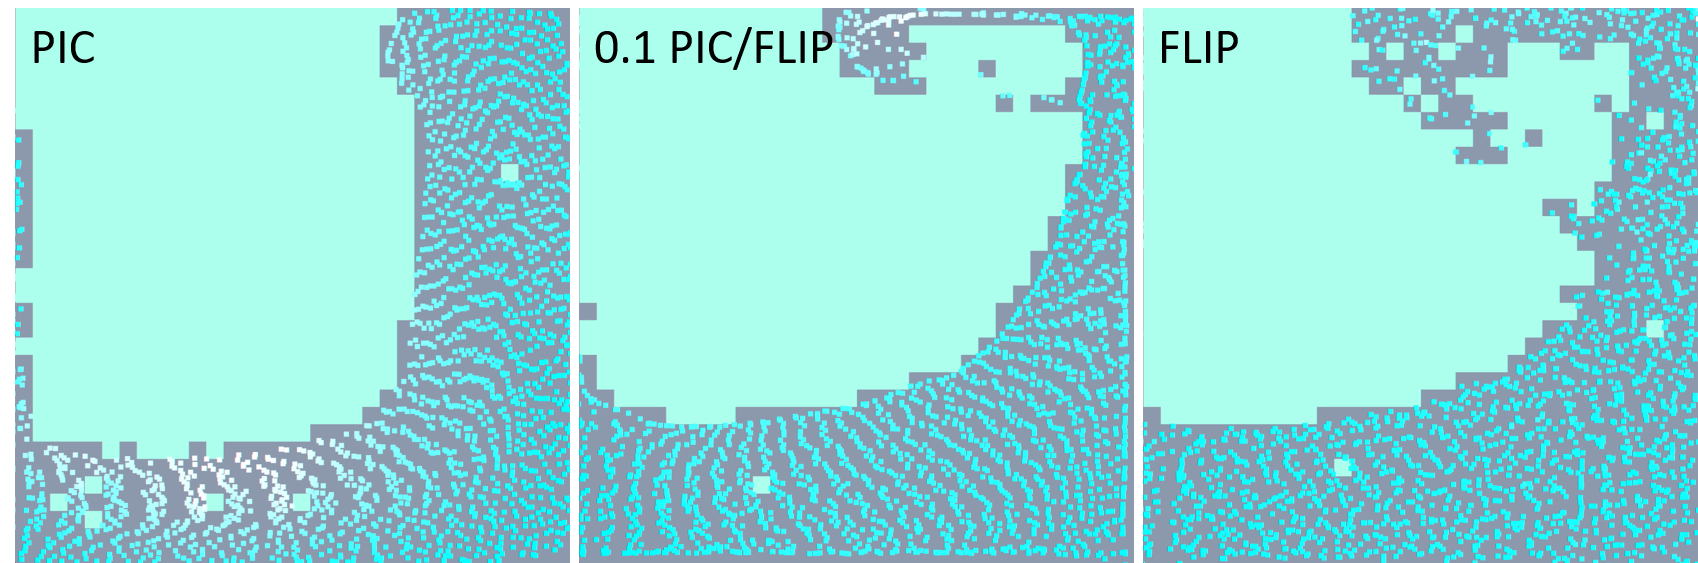
\includegraphics[width=\linewidth]{img/Dam_Break.png}
  \caption{Dam break at $t=0.75$ using (from left to right) PIC, $\alpha{}=0.1$ PIC/FLIP blend, and full FLIP. Full FLIP became unstable and was unable to complete the simulation up to $t=5.0$.} \label{fig:dambreak}
\end{figure}

From the accompanying video, we note as well that the PIC/FLIP blend is much more lively and takes longer to settle into a steady state than PIC. Additionally, we note that because PIC interpolates velocities directly, particles tend to retain their initial configurations relative to their neighbours more, similar to how particles are not free to move relative to each other in solids. By comparison, FLIP as well as the PIC/FLIP blends allow particles to be travelling in different directions, though this raises the implication that the velocity field implied by the particles could be multivariate which also suggests numerical instability.

Other results show similar differences between the three variants. Figure \ref{fig:planks} shows a block of fluid initialized on the top plank and allowed to flow downwards. Again, we see that PIC has a very viscous property, with the fluid dropping from one plank to the other, FLIP is very noisy, and the blend has a good balance. We note that the PIC/FLIP blend demonstrates a good arc as the fluid keeps momentum when dropping from the second plank. A larger $64\times{}64$ resolution version of this same setup is shown on Figure \ref{fig:teaser}.

\begin{figure}[ht]
  \centering
  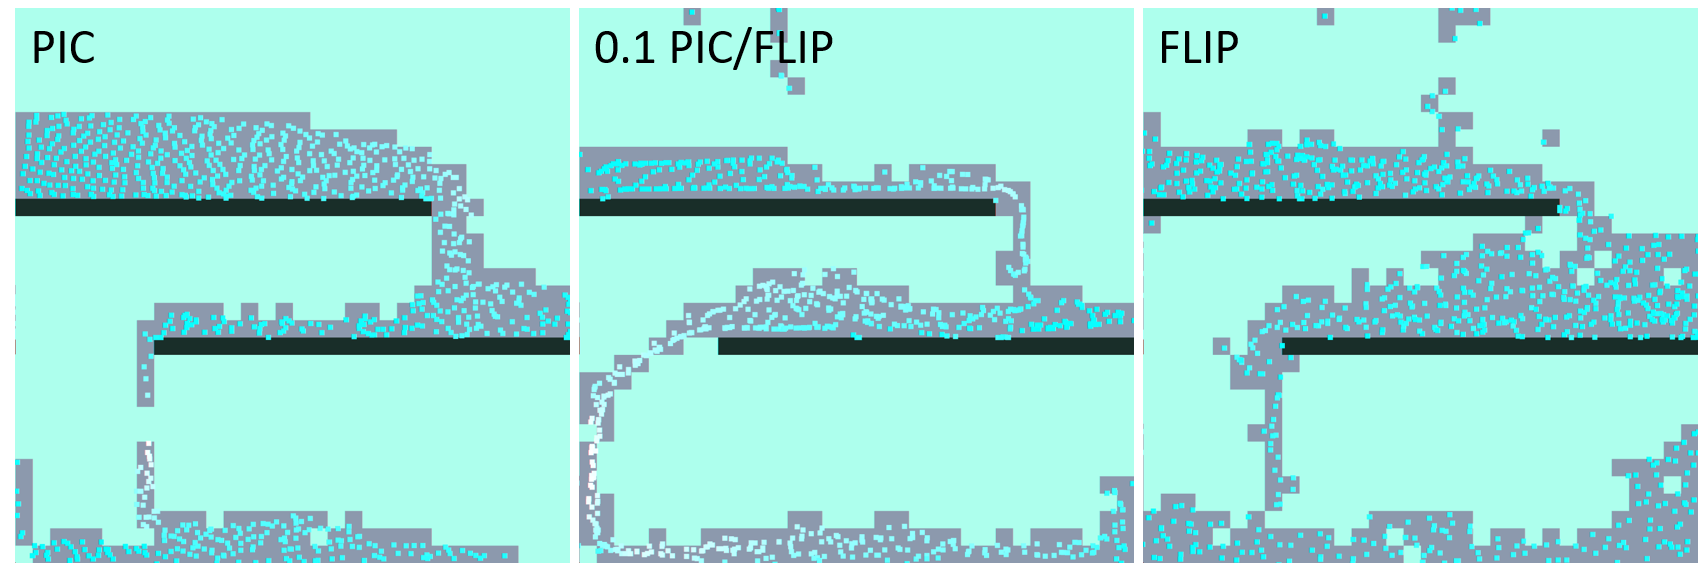
\includegraphics[width=\linewidth]{img/Maze.png}
  \caption{Fluid dropped on two planks at $t=1.5$ using (from left to right) PIC, $\alpha{}=0.1$ PIC/FLIP blend, and full FLIP. Full FLIP became unstable and was unable to complete the simulation up to $t=5.0$.} \label{fig:planks}
\end{figure}

One error we do note, however, is that disconnected pieces of fluid seem to be able to affect each other from afar. For example, falling drops of fluid sometimes slow down before they reach a puddle below. This could be an error in setting up the free surface boundary for the fluid solve, though this would need to be looked into further. Additionally, the solver seems to be handling the left free surfaces incorrectly, which is especially noticable in the fluid block drop as it hits the bottom -- the left free surface seems to slow down while the right free surface retains the correct falling momentum. This, again, could be an error in setting up the boundaries.

To demonstrate slightly more complex boundary interactions, we drop a fluid on a cone-shaped opening as shown on Figure \ref{fig:cone}, using the PIC/FLIP blend. We note that the fluid was able to slowly drain through the opening, creating a stream of fluid that creates waves as it reaches the bottom of the simulation domain.

\begin{figure}[ht]
  \centering
  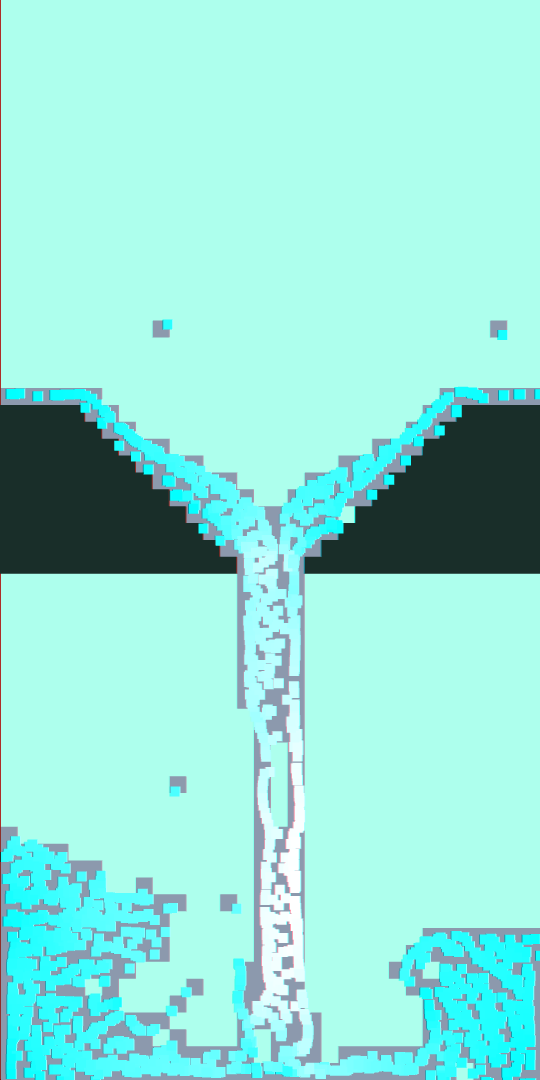
\includegraphics[width=0.35\linewidth]{img/ConeCrop-0.png}
  \caption{Fluid dropped on a cone-shaped opening at $t=0.8$ using $\alpha{}=0.1$ PIC/FLIP blend. A $32\times{}64$ grid was used with timestep size $\Delta{}t=0.001$.} \label{fig:cone}
\end{figure}


\section{Conclusions and Future Work}

We have demonstrated a reasonably working basic implementatiion of a 2D PIC/FLIP fluid solver. There are still a few errors to be solved, as well as additional components to be added to make this solver more fully-featured. In particular, the solver is missing a proper surface reconstruction -- a clear step for improvement would be to implement a level set representation of the surface. More relevant to the MPM scheme itself, the affine transfer of APIC would be a good module to be included in this current implementation \cite{jiang2015}. Once again, improvements to the transfer functions for MPM in general is a fruitful area, with implementation of PolyPIC and MLS-MPM also being feasible \cite{fu2017, hu2018}. Additionally, extending the current solver into 3D may be a useful exercise that greatly increases the solver's utility.

\bibliographystyle{ACM-Reference-Format}
\bibliography{aaatemplate}
\end{document}
